% DalMax README figure: the pool-based active learning loop of the clean campaign.
% Rebuild: see assets/README.md. Self-contained (no images, no external files).
\documentclass[tikz,border=6pt]{standalone}
\usepackage[T1]{fontenc}
\usepackage{helvet}
\renewcommand{\familydefault}{\sfdefault}
\usepackage{amsmath}
\usetikzlibrary{positioning,arrows.meta,shapes.geometric,fit,backgrounds,calc}
\definecolor{cb}{HTML}{1F4E79}  % loop (blue)
\definecolor{cbl}{HTML}{DCE8F3}
\definecolor{co}{HTML}{B4561B}  % query strategy (orange)
\definecolor{col}{HTML}{F6E4D8}
\definecolor{cn}{HTML}{2E6B4F}  % evaluation (green)
\definecolor{cnl}{HTML}{DDEEE5}
\definecolor{cg}{HTML}{4A4A4A}  % neutral (gray)
\definecolor{cgl}{HTML}{EEEEEE}
\tikzset{
  title/.style={draw=#1,fill=#1,text=white,rounded corners=2pt,minimum height=0.75cm,align=center,font=\bfseries,anchor=north west},
  title/.default=cb,
  lstep/.style={draw=cb,fill=cbl,rounded corners=3pt,align=center,inner sep=4pt,text width=3.6cm,minimum height=1.55cm},
  qstep/.style={lstep,draw=co,fill=col,line width=1pt},
  cyl/.style={cylinder,shape border rotate=90,aspect=0.22,draw=#1,fill=#1!12,align=center,minimum height=1.9cm,text width=2.9cm,inner sep=3pt},
  cyl/.default=cb,
  ar/.style={-{Stealth[length=2.6mm]},thick,draw=cb},
  qar/.style={-{Stealth[length=2.6mm]},thick,draw=co},
  lab/.style={font=\footnotesize,text=#1,align=center,fill=white,inner sep=1.5pt},
  lab/.default=cb,
  fam/.style={draw=co,fill=white,rounded corners=2pt,align=left,inner sep=4pt,text width=5.45cm,anchor=north west,minimum height=1.45cm},
  chip/.style={draw=#1,fill=#1!10,rounded corners=2pt,align=left,inner sep=4pt,anchor=north west},
}
\hyphenpenalty=10000 \exhyphenpenalty=10000
\begin{document}
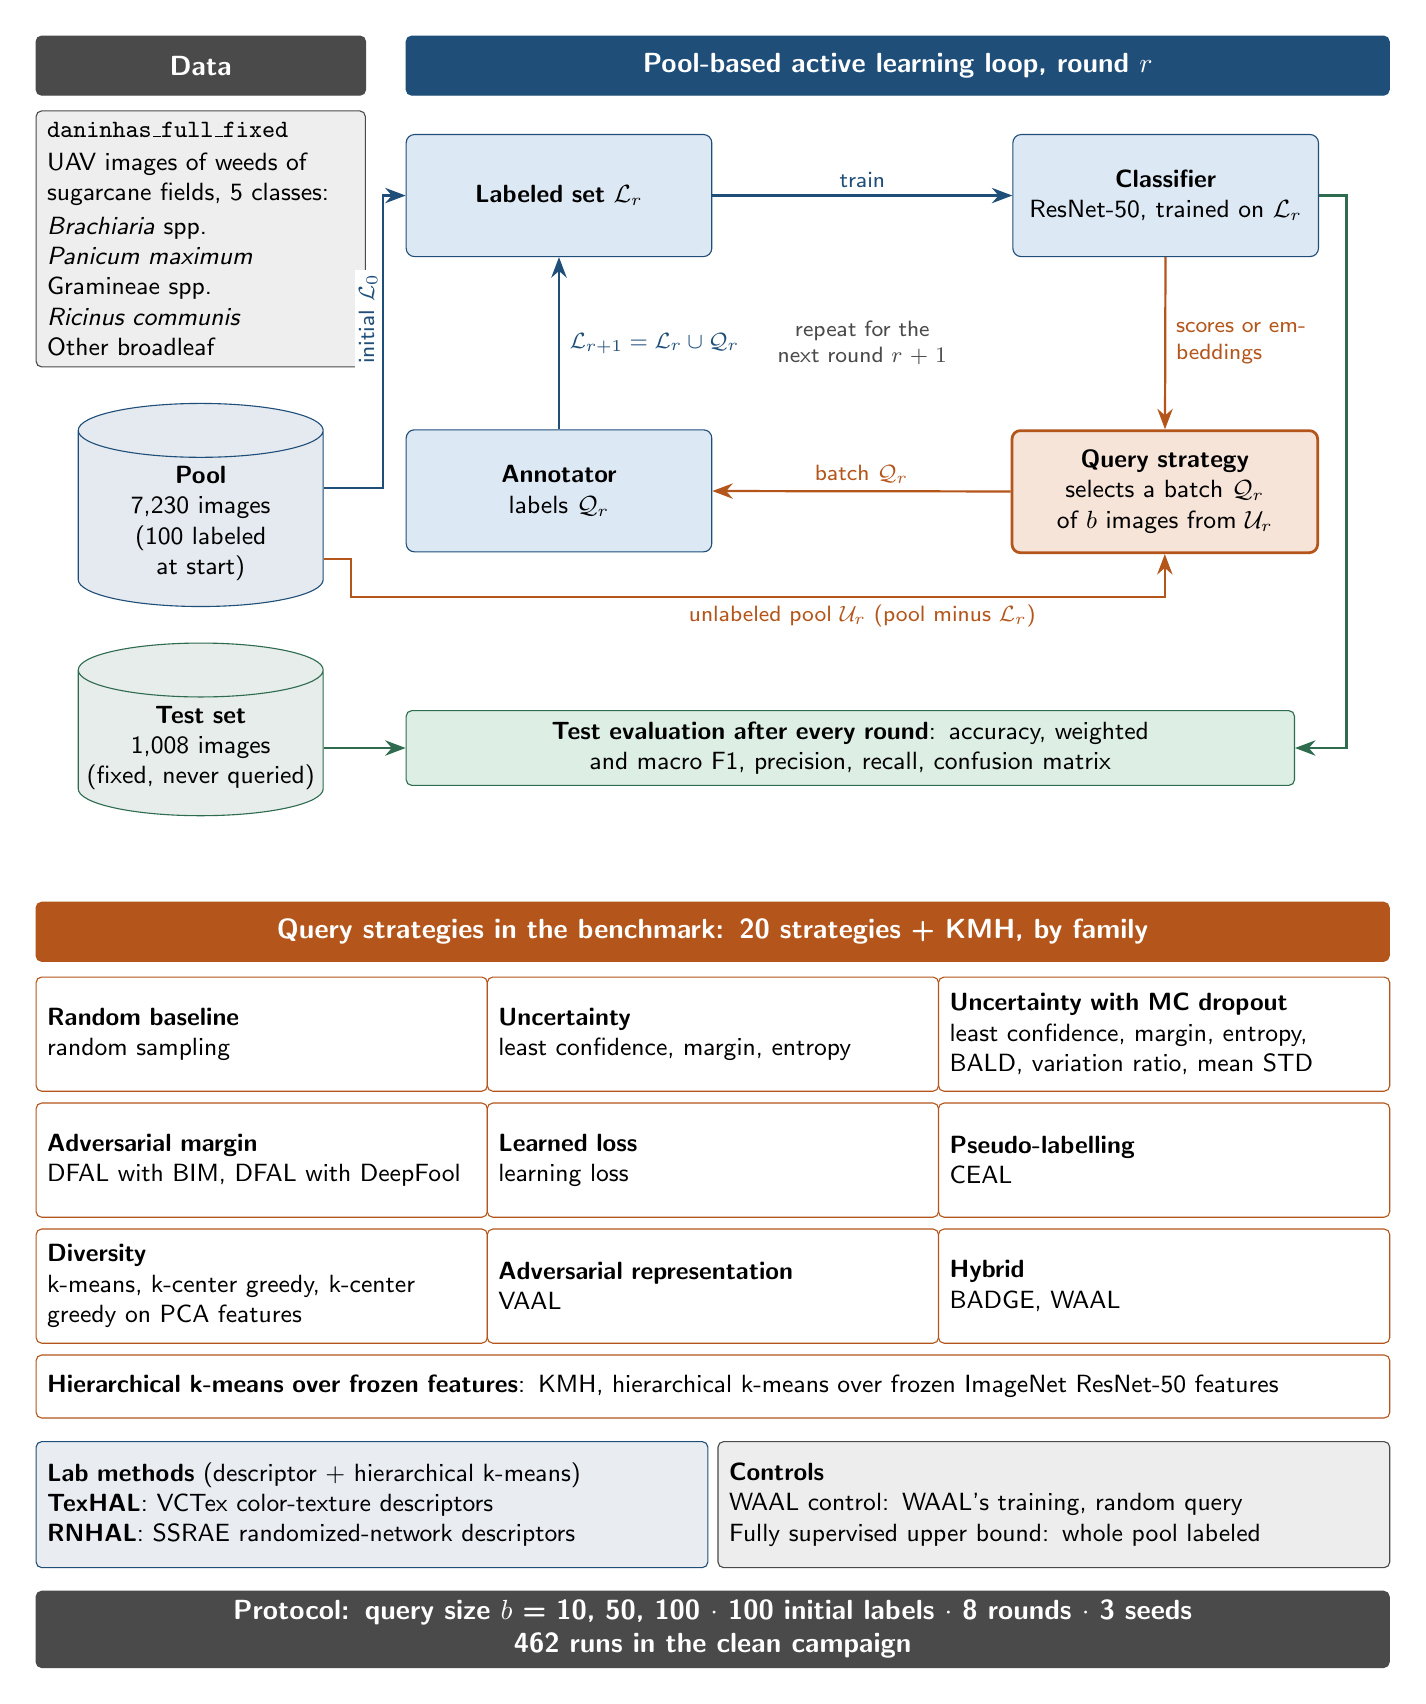
\begin{tikzpicture}[font=\small]
%% white opaque background is added at the end (backgrounds library)

%% ---------------- Data ----------------
\node[title=cg,text width=3.95cm] (td) at (0,0) {Data};
\node[draw=cg,fill=cgl,rounded corners=2pt,align=left,text width=3.9cm,inner sep=4pt,anchor=north west] (ds) at (0,-0.95) {%
{\bfseries\texttt{daninhas\_full\_fixed}}\\[1pt]
UAV images of weeds of sugarcane fields, 5 classes:\\[1pt]
\emph{Brachiaria} spp.\\
\emph{Panicum maximum}\\
Gramineae spp.\\
\emph{Ricinus communis}\\
Other broadleaf};
\node[cyl=cb,anchor=north] (pool) at ($(ds.south)+(0,-0.45)$) {{\bfseries Pool}\\7,230 images\\(100 labeled at start)};
\node[cyl=cn,anchor=north] (test) at ($(pool.south)+(0,-0.45)$) {{\bfseries Test set}\\1,008 images\\(fixed, never queried)};

%% ---------------- Loop ----------------
\node[title,text width=12.25cm] (tl) at (4.7,0) {Pool-based active learning loop, round $r$};
\node[lstep,anchor=north west] (L) at (4.7,-1.25) {{\bfseries Labeled set} $\mathcal{L}_r$};
\node[lstep,anchor=north east] (C) at (16.3,-1.25) {{\bfseries Classifier}\\ResNet-50, trained on $\mathcal{L}_r$};
\node[qstep,anchor=north east] (Q) at (16.3,-5.0) {{\bfseries Query strategy}\\selects a batch $\mathcal{Q}_r$ of $b$ images from $\mathcal{U}_r$};
\node[lstep,anchor=north west] (A) at (4.7,-5.0) {{\bfseries Annotator}\\labels $\mathcal{Q}_r$};
\draw[ar] (L) -- node[lab,above=1pt] {train} (C);
\draw[qar] (C) -- node[lab=co,right=2pt,text width=1.9cm,align=left] {scores or embeddings} (Q);
\draw[qar] (Q) -- node[lab=co,above=1pt] {batch $\mathcal{Q}_r$} (A);
\draw[ar] (A) -- node[lab,right=2pt,text width=2.4cm,align=left] {$\mathcal{L}_{r+1}=\mathcal{L}_r\cup\mathcal{Q}_r$} (L);
\node[align=center,text=cg,font=\footnotesize,text width=3.0cm] at (10.5,-3.9) {repeat for the next round $r+1$};
%% the pool initialises the labeled set
\draw[ar] ($(pool.east)+(0,0.45)$) -- ++(0.75,0) |- (L.west);
\node[lab,anchor=south,rotate=90] at (4.4,-3.6) {initial $\mathcal{L}_0$};
%% the unlabeled part of the pool feeds the query strategy
\draw[qar] ($(pool.east)+(0,-0.45)$) -- ++(0.35,0) |- ($(Q.south)+(0,-0.55)$) -- (Q.south);
\node[lab=co,anchor=north] at (10.5,-7.17) {unlabeled pool $\mathcal{U}_r$ (pool minus $\mathcal{L}_r$)};
%% the classifier of every round is evaluated on the fixed test set
\node[draw=cn,fill=cnl,rounded corners=2pt,align=center,text width=11.0cm,inner sep=4pt,anchor=west] (ev) at (test.east -| L.west) {{\bfseries Test evaluation after every round}: accuracy, weighted and macro F1, precision, recall, confusion matrix};
\draw[ar,draw=cn] (test.east) -- (ev.west);
\draw[ar,draw=cn] (C.east) -- ++(0.35,0) |- (ev.east);

%% ---------------- Strategy families ----------------
\node[title=co,text width=16.95cm] (tf) at (0,-11.0) {Query strategies in the benchmark: 20 strategies + KMH, by family};
\def\fy{-11.95}
\def\fya{-13.55}
\def\fyb{-15.15}
\node[fam] at (0,\fy)      {{\bfseries Random baseline}\\random sampling};
\node[fam] at (5.73,\fy)   {{\bfseries Uncertainty}\\least confidence, margin, entropy};
\node[fam] at (11.46,\fy)   {{\bfseries Uncertainty with MC dropout}\\least confidence, margin, entropy, BALD, variation ratio, mean STD};
\node[fam] at (0,\fya)     {{\bfseries Adversarial margin}\\DFAL with BIM, DFAL with DeepFool};
\node[fam] at (5.73,\fya)  {{\bfseries Learned loss}\\learning loss};
\node[fam] at (11.46,\fya)  {{\bfseries Pseudo-labelling}\\CEAL};
\node[fam] at (0,\fyb)     {{\bfseries Diversity}\\k-means, k-center greedy, k-center greedy on PCA features};
\node[fam] at (5.73,\fyb)  {{\bfseries Adversarial representation}\\VAAL};
\node[fam] at (11.46,\fyb)  {{\bfseries Hybrid}\\BADGE, WAAL};
\node[fam,text width=16.91cm,minimum height=0.8cm] at (0,-16.75) {{\bfseries Hierarchical k-means over frozen features}: KMH, hierarchical k-means over frozen ImageNet ResNet-50 features};

%% ---------------- Lab methods and controls ----------------
\node[chip=cb,text width=8.25cm,minimum height=1.6cm] (lm) at (0,-17.85) {{\bfseries Lab methods} (descriptor + hierarchical k-means)\\\textbf{TexHAL}: VCTex color-texture descriptors\\\textbf{RNHAL}: SSRAE randomized-network descriptors};
\node[chip=cg,text width=8.25cm,minimum height=1.6cm] (ct) at (8.66,-17.85) {{\bfseries Controls}\\WAAL control: WAAL's training, random query\\Fully supervised upper bound: whole pool labeled};

%% ---------------- Protocol ----------------
\node[title=cg,text width=16.95cm,minimum height=0.85cm] (tp) at (0,-19.75) {Protocol: query size $b$ = 10, 50, 100 $\cdot$ 100 initial labels $\cdot$ 8 rounds $\cdot$ 3 seeds\\462 runs in the clean campaign};

\begin{scope}[on background layer]
  \fill[white] ($(current bounding box.south west)+(-0.1,-0.1)$) rectangle ($(current bounding box.north east)+(0.1,0.1)$);
\end{scope}
\end{tikzpicture}
\end{document}
